\chapter{Implementation}
This chapter serves to discuss the implementation specifics of the design of my application, including the development environment and any issues I encountered in implementing the features set out in my project objectives.

\section{Development Environment}
The application was developed primarily on a Fujitsu Lifebook A series with an Intel i5-3230M CPU @ 2.60GHz processor, 4GB of RAM and running Windows 10. The code was developed using Jet Brains IntelliJ IDE and Google Chrome developer console.

\section{Features}
\subsection{Reading User Input}
\subsubsection{Implementation}
The user input was one of the first parts of the application to be implemented, and consisted of reading in a .fa FASTA file and just outputting the content of the file to the console and return it from the method to be tested against with automated unit tests. It was developed further to extract out the header, checking that it began with the `\textgreater ' character and then every other line was included as part of that contig. 

Originally it dealt with only one contig at a time, but was then expanded to be able to read in a full list of contigs and separate them based on where the header line starts. The code was eventually modified so that the user could paste data, that would be broken into components and processed in the same way. This was for the pasting of the user data rather than file upload, as I decided I would rather have pasted data than uploads for the current state of the application.

\begin{figure}[H]
\centering
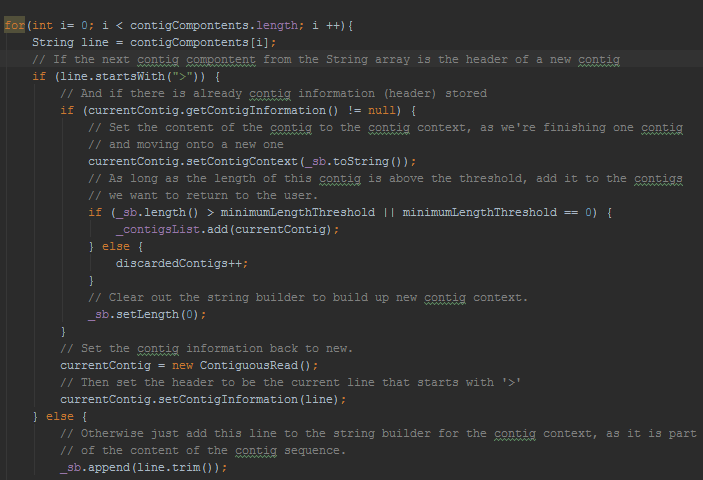
\includegraphics[width=0.9\textwidth]{images/readuserdata}
\caption{Part of the code for reading in a users data when they have pasted it into the text area of the web service. Deals with creating new ContiguousRead objects and adding them to a ContigResult every time it finds a new header for a contig (or reaches the end of the input).}
\end{figure}

\subsubsection{Issues}
It took some time to deal with the formatting of the file and knowing when one contiguous read starts and one ends. There was some issue with the escape/return characters in the dealing of pasted content by a user, but this was solved by breaking the pasted content into an array of its components.

While not an issue as such, the original version of the application would carry out the quality assessment of each contig as and when they were read in, to avoid holding too much data in memory. As the design evolved this was no longer a possibility, as it didn't allow the user to see their contigs before they were processed, or do any additional inspection on the contigs without holding the entire user data submitted in memory and going through it a second time upon an inspection request to find the contig they wanted. This option is still a possibility, but is an optimization aspect that wasn't in scope for the project. Additionally, the separation of responsibilities is better in this version of the code after being refactored from the time when the read class both read and assessed the contigs.

It did take longer to implement this than I had anticipated due to me changing from file reading to user pasting, and trying to find contig start and ends to read in the data versus read and assess at the same time.

\subsection{Counting GC Content \& Percentage}
\subsubsection{Implementation}
Counting the GC content of the application involved breaking up the contig characters into sizes based on the set window length by the user, then working out the percentage of G and C characters in each of those windows. Each part of the contig that is split is put into a `GcWindow' object, that has methods for counting the number of G and C characters within it.

\begin{figure}[H]
\centering
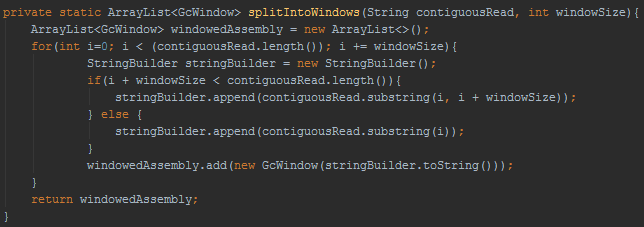
\includegraphics[width=0.9\textwidth]{images/splitgcwindows}
\caption{The code for splitting a contiguous read into windows available for calculating the GC content window percentages.}
\end{figure}

Once split, the GcWindows are passed to have their percentages calculated and added to an ArrayList of Doubles This is used for calculation with the mean, standard deviation and for returning results to the user for use in the View.

\begin{figure}[H]
\centering
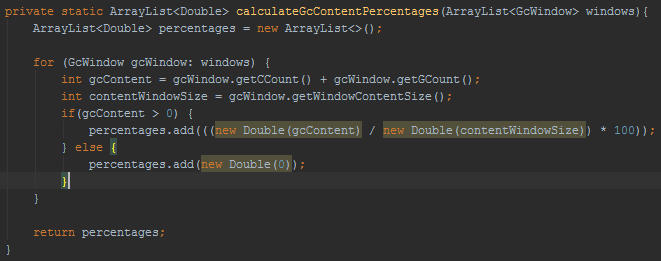
\includegraphics[width=0.9\textwidth]{images/calcgcpercentage}
\caption{The code for calculating the GC content percentages for each window passed into the method.}
\end{figure}

\subsubsection{Issues}
In principle this is, and was, an easy task, yet took me longer to complete because my domain knowledge was still somewhat lacking and I got caught up on the little details that kept me from progressing, even though I didn't need to know of them or use them in the process of working out the GC content windows. Overall there were no issues with the implementation once I got my head around why it was worth doing this and how it should be presented as a quality measure to the user.

\subsection{Displaying GC Content percentage}
\subsubsection{Implementation}
I began to attempt to implement GC content viewing with Plotly.js right from the beginning, and so I had a prototype up and running fairly quickly where I manually took the results from the console output of the Java application and pasted them into the final containing my Plotly.js prototype to be used as data. 

Next I worked this in with Thymeleaf to get the results directly from my Java application, then turned them into JavaScript and used the data from that for the chart. The x axis labeling for the chart is manually created in order to represent where the GC window for each bar starts and finishes. The earlier design had window numbers along the x-axis, populated by Plotly.js. These were of no use to a user though, as if they wanted to find out what GC window they were looking at they would have to manually work out where the window started and ended from their window size multiplied by the window number of interest.

\begin{figure}[H]
\centering
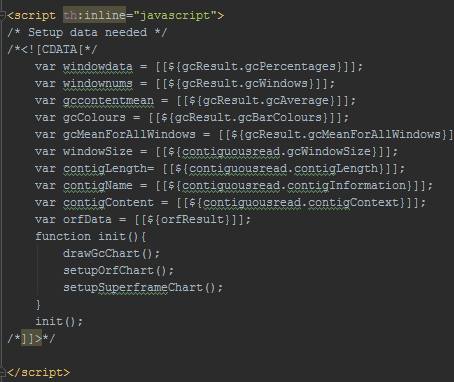
\includegraphics[width=0.6\textwidth]{images/thymeleafdata}
\caption{Extracting the data from the Model, provided by the Controller to the View, using Thymeleaf's inline tag to be able to use CDATA to convert the Thymeleaf extracts into JavaScript.}
\end{figure}

The red bars of the GC chart displaying where the percentage of a window is over or under the threshold of the mean of all GC window percentages was implemented as a useful aid to the user, and the colours are set in the Model rather than made in the View. The reasoning for this was to implement a system that would provided the View with what it needed and not needing the View to calculate anything, only consume the values (in this case the GC window data and RGB data) to display results.

\begin{figure}[H]
\centering
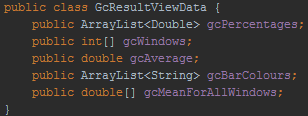
\includegraphics[width=0.6\textwidth]{images/gcviewdata}
\caption{`GcContentViewData', the object provided to the View in order to display the GC content data to the user.}
\end{figure}

The final thing to add was the Mean line. This is just displaying to the user where the mean of all the GC windows lie, and helps with the visualization of if any windows of their contiguous read look like they might have issues.
\subsubsection{Issues}
The main issue I had with displaying the GC content percentages with Plotly.js was getting data to actually display as I was unfamiliar with Plotly.js and Thymeleaf once I started using Spring Boot. Thymeleaf makes getting data from the Objects in the Model very easy and simple, but since I was trying to integrate two technologies together that I had never used before, it took some time to find the right way of accessing the data from my Object through Thymeleaf, into JavaScript and then the correct format for use by Plotly.js.

The next issue was trying to get the line for the Mean to show. The way I got this to work was using an additional data input for the same chart as displaying the GC content window bars and having the same number of data points as there are GC windows, where each data point is the mean number, in order to get the chart to display a line across the entire chart to match the GC windows.

\subsection{Finding Open Reading Frames}
\subsubsection{Implementation}
The implementation of Open Reading Frames happened in a few steps, with the design and code evolving as I understood more what they were and how best to present the results. At first, I was only finding a single, longest ORF Location, as I did not fully comprehend what an ORF was. This was just looking at a contig and finding the first start Codon of ATG and the last stop Codon of TAG/TAA/TGA. Once I understood them though, the process became about how to find whatever ORF Locations I could. Using Test Driven Development was extremely useful for this step, as I wrote tests for finding specific ORF Locations in small sequences I created myself and ran the code against them.

After a number of attempts at trying to find the ORF Locations within a contig frame, I settled on a method of going through the entire frame, breaking it up into characters of 3 and only keeping the start and stop Codons in lists of each. Each Codon was stored with data about where it starts and ends, in order to be able to later reconstruct the contig between a start and stop Codon based on the character positions.

\begin{figure}[H]
\centering
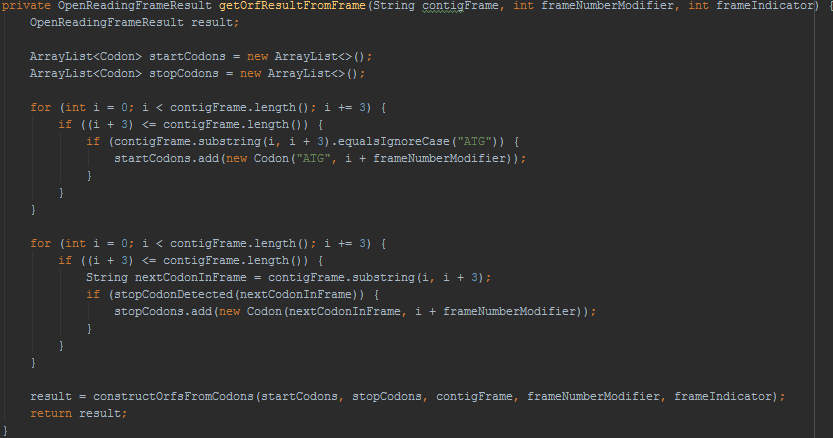
\includegraphics[width=0.9\textwidth]{images/orffind2}
\caption{Finding all of the start and stop Codons from within the passed frame from the contig.}
\end{figure}


Each frame is separated by creating a substring of the original contiguous read, removing 0, 1 and then 2 characters for the first three frames, and the same for the reverse frames but with the contiguous read sequence reversed with the opposing base pair of each character used. 

\begin{figure}[H]
\centering
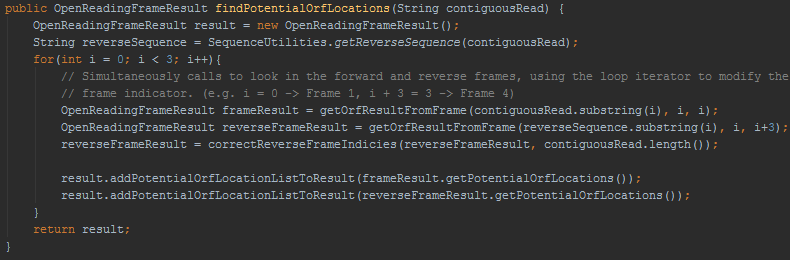
\includegraphics[width=0.9\textwidth]{images/orffind1}
\caption{Extracting each frame and calling to run the ORF Finding process.}
\end{figure}

For each ORF Location found in a reverse frame, the start and stop indexes are swapped, representing that what is the `Start' of an ORF Location is actually closer to the end of the contiguous read. This is so that it can be displayed appropriately in the View, and match up with the proper direction with the forward frames.

\begin{figure}[H]
\centering
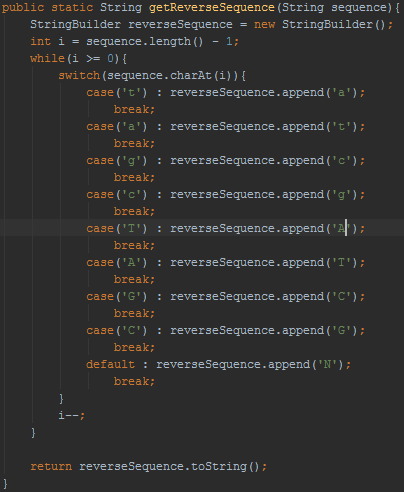
\includegraphics[width=0.6\textwidth]{images/orffind4}
\caption{Getting the base pair characters of a reverse frame is as simple as a switch statement and building the reversed contig from back to front.}
\end{figure}

Through this process, it made it possible to find which Codons came before and after which within the contiguous read in order to find which would construct the longest ORF Locations, which Start Codons were redundant (as they were between an earlier start Codon and the next Stop Codon), and in my first completed version of the algorithm, where the last Stop Codon before the next Start Codon was.

At this time, I still had a misunderstanding about protein coding regions, in that I believed the end of an ORF Location was at the last stop Codon before the next start Codon, when in fact it should have been the first stop Codon it reaches is the end of the current Codon. This was a simple fix though as it just involved removing a section of my code and fixing my tests.

\begin{figure}[H]
\centering
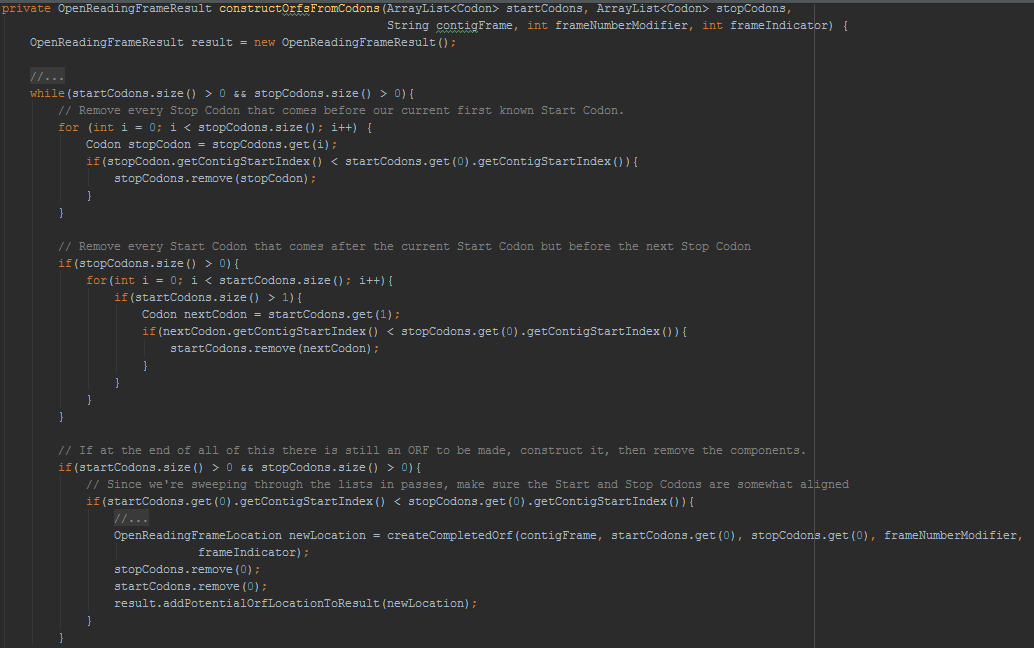
\includegraphics[width=0.9\textwidth]{images/orffind3}
\caption{`Zipping' together ORF Locations from start and stop Codons within the frame.}
\end{figure}

Once each frame has been processed to find the ORF Locations within them, the results of each frame are combined together in a single OpenReadingFrameResult. Each ORF Location is aware of what frame it belongs to, and so combining them all into one result doesn't make a difference when determining what ORF Location belongs where.

\subsubsection{Issues}
The two main issues with implementing the Open Reading Frame finding algorithms were my lack of understanding of what they were when I began, leading to the second issue of implementing more than was necessary. It took me longer than I had anticipated to implement the code for finding ORF Locations because I believed I had the additional requirement task of finding the last stop Codon before the next start Codon, where every stop Codon between the initial start Codon and that last stop Codon was to be included in the ORF Location but ignored as an actual start and stop.

Thinking up how to do this algorithmically took some planning and time, and eventually I came to the conclusion of finding all start and stop Codons and then running a while loop, checking that there was at least 1 of each left in each list to make an ORF Location, where the Start came after the Stop (for reverse frames, this logic still applies as the indexes are only reverse after the ORF Locations have been constructed) and then carrying out a number of conditional checks to remove any start and stop Codons that came between the longest ORF that could possibly be made.

Once I had realized this was erroneous and the first stop Codon encountered is the actual end of an ORF Location and not to continue, it was too late to recover any time and I just had to remove the code that caused the issue and rewrite my tests to match the actual expected outcome. Aside this, once I designed the code based around the `zipping' of start and stop Codons together, the implementation was relatively simple, using unit tests to ensure I was correctly implementing the algorithm for expected results.

\subsection{Displaying ORF Locations}
\subsubsection{Implementation}
The first part of the ORF Location displaying for the View takes place in the Controller, where it strips away ORF Locations under minimum length threshold set by the user and then sorts all ORF Locations by length using a comparison method. The display of the ORF Locations in their particular frames is done using HTML5 Canvas, one for each frame. As each ORF Location holds an integer value representing what frame it belongs to, when painting the canvases it is a simple matter finding the correct context  for the particular frame from an array of canvas contexts
\begin{verbatim}
var currentContext = contextList[orfData[i].frameIndicator];
\end{verbatim}
Reverse and forward frame ORF Locations are painted in the same way, except the start and stop indexes are swapped for reverse frames. Likewise, for the highlighted ORF Location to be painted, the only difference is that the current highlighted frame is stored in a global variable (updated any time an ORF Location is clicked in the list or on a frame) and when re-painting the frame canvases and iterating through the list of ORF Locations, when the loop reaches that ORF Location the fill colour is set to be different than every other ORF Location.

Finding a click within a canvas frame is as simple as checking if the click is horizontally within a frame location by calculating where the start and stop points of all the ORF Locations (with that frame in particular) are and if the click falls within one of the the ORF Locations.

\begin{figure}[H]
\centering
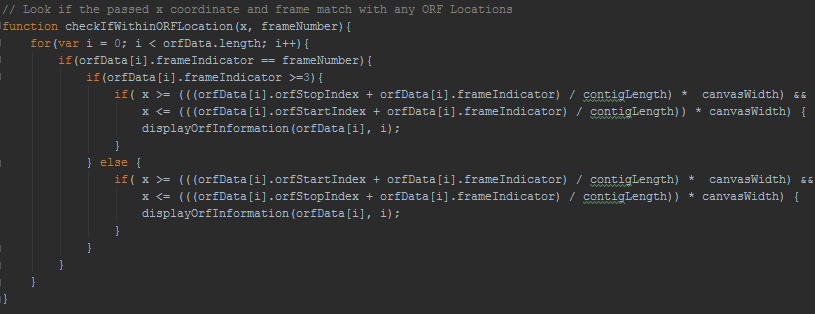
\includegraphics[width=0.9\textwidth]{images/orfdisplay1}
\caption{Finding if a click if within an ORF Location is as simple as going through the list of ORF Locations, only checking against those within the same frame as the click, then looking at whether the click is within the start and stop points of an ORF Location within the canvas, based on the size and location of where it was painted (for reverse frames, the start and stop points are swapped, as reverse frames are displayed in the same direction as forward frames, with the indexes in the right order for a reverse frame).}
\end{figure}

\subsubsection{Issues}
Implementation through each ORF Location knowing where it starts and ends, the characters between in a list. Each has a frame indicator, allows them to be kept in a single array. Javascript goes through the list and uses HTML5 canvas to draw them out in 6 different canvases. Working on finding user clicks within the canvas objects, getting data from Thymeleaf to display it from the Objects. Formatting the display and using colour to highlight the start and stop codons.
Issues included finding the clicks, highlighting both the menu and the item on canvas. Took some time to get the formatting in the table correct

\subsection{Superframe Comparisson}
\subsubsection{Implementation}
\subsubsection{Issues}
Making the view of superframe to help the user compare the ORF and GC content. Able to be built upon with k-mer frequency analysis and other techniques as added. The overall 'compare all' chart. Borrowed code from the ORF canvases. Breaking things up into windows from the GC content.

Not really any issues, just trying to find the best way to display it to the user and convey any areas where things don't line up properly. Would like to work on this more and develop a system to detect where the issues really are. Need more techniques.

\subsection{User Interface Organisation}
\subsubsection{Implementation}
\subsubsection{Issues}
User input section originally having all parameters was messy, only dealing with one contig, then multiple contigs, having parameters appear underneath any contig you wish to inspect, having all charts on the toolbox page displayed in one long list looked ugly, implemented tabs from (credit to the guy here).

\subsection{Implementation Review}
Found that GC Content percentage and ORF Location finding took a lot longer than expected, especially considering that I implemented an additional part of ORF Finding that wasn't needed, and got refactored 3 times until I reached that point. Delayed me to the point I felt I wouldn't have time to implement k-mer frequency analysis. 
User interface design and programming also took a lot longer. Wanted to present the information in a clean and useful way, without cluttering the page. Getting used to Thymeleaf and how it took the data from the Objects took a while to get used to. Felt that my implementation process was acceptable but issues slowed me down significantly. Everything else I felt I would implement got implemented, but the Superframe needs additional consideration. A lot of the quality assessment is still on the user to look at the produced reports and their content to consider whether they themselves feel their assembly file is good or not through factors highlighted by my application.

% The implementation should look at any issues you encountered as you tried to implement your design. During the work, you might have found that elements of your design were unnecessary or overly complex; perhaps third party libraries were available that simplified some of the functions that you intended to implement. If things were easier in some areas, then how did you adapt your project to take account of your findings?

% It is more likely that things were more complex than you first thought. In particular, were there any problems or difficulties that you found during implementation that you had to address? Did such problems simply delay you or were they more significant? 

% You can conclude this section by reviewing the end of the implementation stage against the planned requirements. 
